\documentclass[onecolumn, draftclsnofoot,10pt, compsoc]{IEEEtran}
\usepackage{graphicx}
\usepackage{url}
\usepackage{setspace}
\graphicspath{ {images/} }

\usepackage{geometry}
\geometry{textheight=9.5in, textwidth=7in}

\def \CapstoneTeamName{		Look Boss, No Hands}
\def \CapstoneTeamNumber{		9}
\def \GroupMemberOne{			Brandon Dring}
\def \GroupMemberTwo{			Nipun Bathini}
\def \GroupMemberThree{			Carl Benson}
\def \CapstoneProjectName{		CDK Global: No more touch. No more Keyboard. Bring it All Together. Using Technology to Teach Humans.}
\def \CapstoneSponsorCompany{	CDK Global}
\def \CapstoneSponsorPerson{		Trevor moore}


\def \DocType{Problem Statement}

\newcommand{\NameSigPair}[1]{\par
\makebox[2.75in][r]{#1} \hfil 	\makebox[3.25in]{\makebox[2.25in]{\hrulefill} \hfill		\makebox[.75in]{\hrulefill}}
\par\vspace{-12pt} \textit{\tiny\noindent
\makebox[2.75in]{} \hfil		\makebox[3.25in]{\makebox[2.25in][r]{Signature} \hfill	\makebox[.75in][r]{Date}}}}


%%%%%%%%%%%%%%%%%%%%%%%%%%%%%%%%%%%%%%%
\begin{document}
\begin{titlepage}
    \pagenumbering{gobble}
    \begin{singlespace}
        \hfill
        \par\vspace{.2in}
        \centering
        \scshape{
            \huge CS Senior Capstone \DocType \par
            {\large October 27th, 2017, Fall 2017}\par
            \vspace{.5in}
            \textbf{\Huge\CapstoneProjectName}\par
            \vspace{.25in}
              

            {\large Prepared for}\par
            \Huge \CapstoneSponsorCompany\par
            \vspace{10pt}
            {\Large\NameSigPair{\CapstoneSponsorPerson}\par}
            \vspace{10pt}
            {\large Prepared by }\par
            Group\CapstoneTeamNumber\par
            % 5. comment out the line below this one if you do not wish to name your team
            \vspace{0.2cm}
            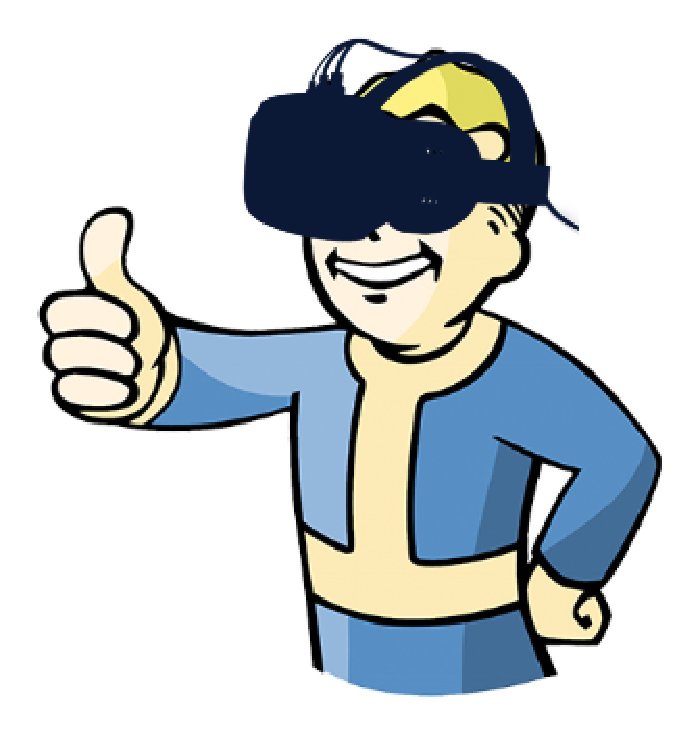
\includegraphics[height=4cm]{Team-Logo}\\
            \vspace{0.2cm}
            \CapstoneTeamName\par
            \vspace{5pt}
            
            \vspace{45pt}
            {\Large
                \NameSigPair{\GroupMemberOne}\par
                \NameSigPair{\GroupMemberTwo}\par
                \NameSigPair{\GroupMemberThree}\par
            }
            \vspace{10pt}
        }
        \begin{abstract}
        % 6. Fill in your abstract
        Look Boss, No hands seeks to develop a new interaction method between a user looking at enterprise data. Instead of sitting behind a computer screen typing and clicking around to get graphs, and charts. This project aims to remove the standard methods of input, in lieu of more novel methods of input such as, voice and virtual reality. With the stretch goals of tracking a user's interaction with the new experience via a wearable.



        \end{abstract}
    \end{singlespace}
\end{titlepage}
\newpage
\pagenumbering{arabic}
\tableofcontents
\clearpage

%%%%%%%%%%%%%%%%%%%%%%%%%%%%%%%%%%%%%%%%%%%%%%%%%%%%%%%%%%%%%%%%%%%%%%%%%%%%%%

\section{Introduction}
    \subsection{Purpose}
        The purpose of this document is to provide the specific requirements needed to our client (Trevor Moore), about the Look Boss, No Hands project, and what it means to be done and to succeed. 
    
    \subsection{Scope}
        The Look Boss, No Hands software will allow for voice recognition to retrieve data and show it in a human comprehensive way with data visualization on a VR headset. This allows for the integration of three separate systems to integrate with one to provide users a new method of access and interaction with data.
    
    \subsection{Definitions, Acronyms, Abbreviations}
    
    \begin{center}
        \begin{tabular}{|c| c| c|}
            \hline
            VR & Virtual Reality \\
            \hline
            Client & Trevor Moore \\
            \hline 
            Project & Look Boss, No Hands \\
            \hline
            Wearables & Fitbit like device that is worn on the wrist and is able to track someones heart rate and relay it back to a phone.\\
            \hline
        \end{tabular}
    \end{center}
    
    \subsection{References}
        IEEE 830-1998
    
    \subsection{Overview}
        The rest of this document contains descriptions of the required functionality, interfaces, and use cases.
    \section{Overall Description}
    
    \subsection{Product perspective}
        The product is intended to provide an interface for accessing a database and displaying retrieved data in a VR headset. Due to this, the system is not self-contained. The project is also built on the assumption that a user doesn’t have to use their hands to interact with a computer, instead using their voice to be put inside a virtual environment to experience the data.
    
    \subsection{Product Functions}
    
        \subsubsection{Voice Recognition}
            Voice recognition is one of the two primary functions of the product. This lets a user verbally request data. At the very least, it needs to be able to take in one command that correlates to the data desired. Such as ``Show me Ford’s sales data in 2016``. 
    
        \subsubsection{Display}
            Display is the other primary function. The display in VR should show a user data in a virtual environment. In which they can interact with the data such that they can overlay graphs, zoom in and out between time. 
    
        \subsubsection{Secondary Commands And Displays (Stretch Goal)}
            Adding a secondary command will show how modular our system is, and the ease of adding another query actually is. 
        
        \subsubsection{Heart Rate Monitoring}
            A user wearing a wearable will have their heart rate monitored and tracked by the device, learning what data trends causes stress in the user and to later send notifications when the data begins following a similar trend. 
        
    \subsection{User Characteristics}
        Everyone should be able to experience the program by putting on the headset and telling the voice assistant to do something. 
    
    \subsection{Constraints}
        There should only be a certain number of ways someone can request the voice assistant to do something. Based on the ambiguity of the English language.

    \subsection{Assumptions and Dependencies}
        The entire project relies on a powerful enough computer to be able to run a VR system. And that the computer is able to properly connect to the server awaiting signals to populate the headset with an environment. 

\section{Specific Requirements}
    \subsection{External Interface Requirements}
        \subsubsection{System Interfaces}
            \begin{itemize}
                \item The product needs to interface with a database in order to retrieve data
                \item Speech recognition in order to determine what data should be retrieved
            \end{itemize}
        \subsubsection{User Interfaces}
            \begin{itemize}
                \item A user uses their voice to verbally request data to be shown. A user can request data to view by simply putting on the headset and speaking
                \item A VR headset to display the requested data
            \end{itemize}
            
            \subsubsection{Hardware Interfaces}
            \begin{itemize}
                \item The user should be able to just simply slip on the headset, tell the voice assistant to do something, and then see it in VR.
            \end{itemize}
            
            \subsubsection{Communications Interfaces}
            \begin{itemize}
                \item The entire project is based on communication, such that a user speaks to the voice assistant to request data, and the VR headset places the user in the virtual environment. 
            \end{itemize}
            
    \subsection{Functional Requirements}
    
        \subsubsection{Voice Assistant}
            Introduction / Purpose
            \begin{itemize}
                \item The voice assistant be the main input method of taking in commands and starting the appropriate programs.
            \end{itemize}
            Response Sequence
            \begin{itemize}
                \item The voice assistant should state that it got the command received, and reply back letting the user know that the correct program has been started.
            \end{itemize}
            Associated Functional Requirements
            \begin{itemize}
                \item (Stretch Goal) should the project be finished semi-early, the next step would be adding more commands to the voice assistant to process. 

            \end{itemize}
        \subsubsection{VR Headset}
            \begin{itemize}
                    \item The headset should be synchronized with the voice assistant to respond and show the appropriate data visualization when prompted. In which a user can reach out and touch and move the data with the hand controllers. 
            \end{itemize}
    
    \subsection{Design Constraints}
        Our client has stated that while the base goal of using an Alexa to request data from words. The system must be modular and flexible enough to incorporate new commands to pull from the database and display to the VR with minimal effort. Meaning adding new commands shouldn’t take more than a few hours worth of work both on the voice recognition and virtual reality side. 

    
    \subsection{Software System Attributes}
        The code must be testable and tested for any pull request that is to be added to the master branch.
    
    %\subsection{Other Requirements}

\section{Non-Functional Requirements}

\subsection{Performance requirements}
    A user should simply be able to walk into a pre-configured environment, and speak a command to the voice assistant. The process of populating the VR headset shouldn't take more than 15 seconds. 
\subsection{Software Quality}
   The software quality of our product must allow for further addition of more data from multiple other dealerships. Employees will have to add additional data as new dealerships rise. To allow easy modifications, our code must be uniformed and simple to understand. As employees add more data to the databases, more information can be retrieved from the voice assistant to the VR headset.  

\section{Gantt Chart}
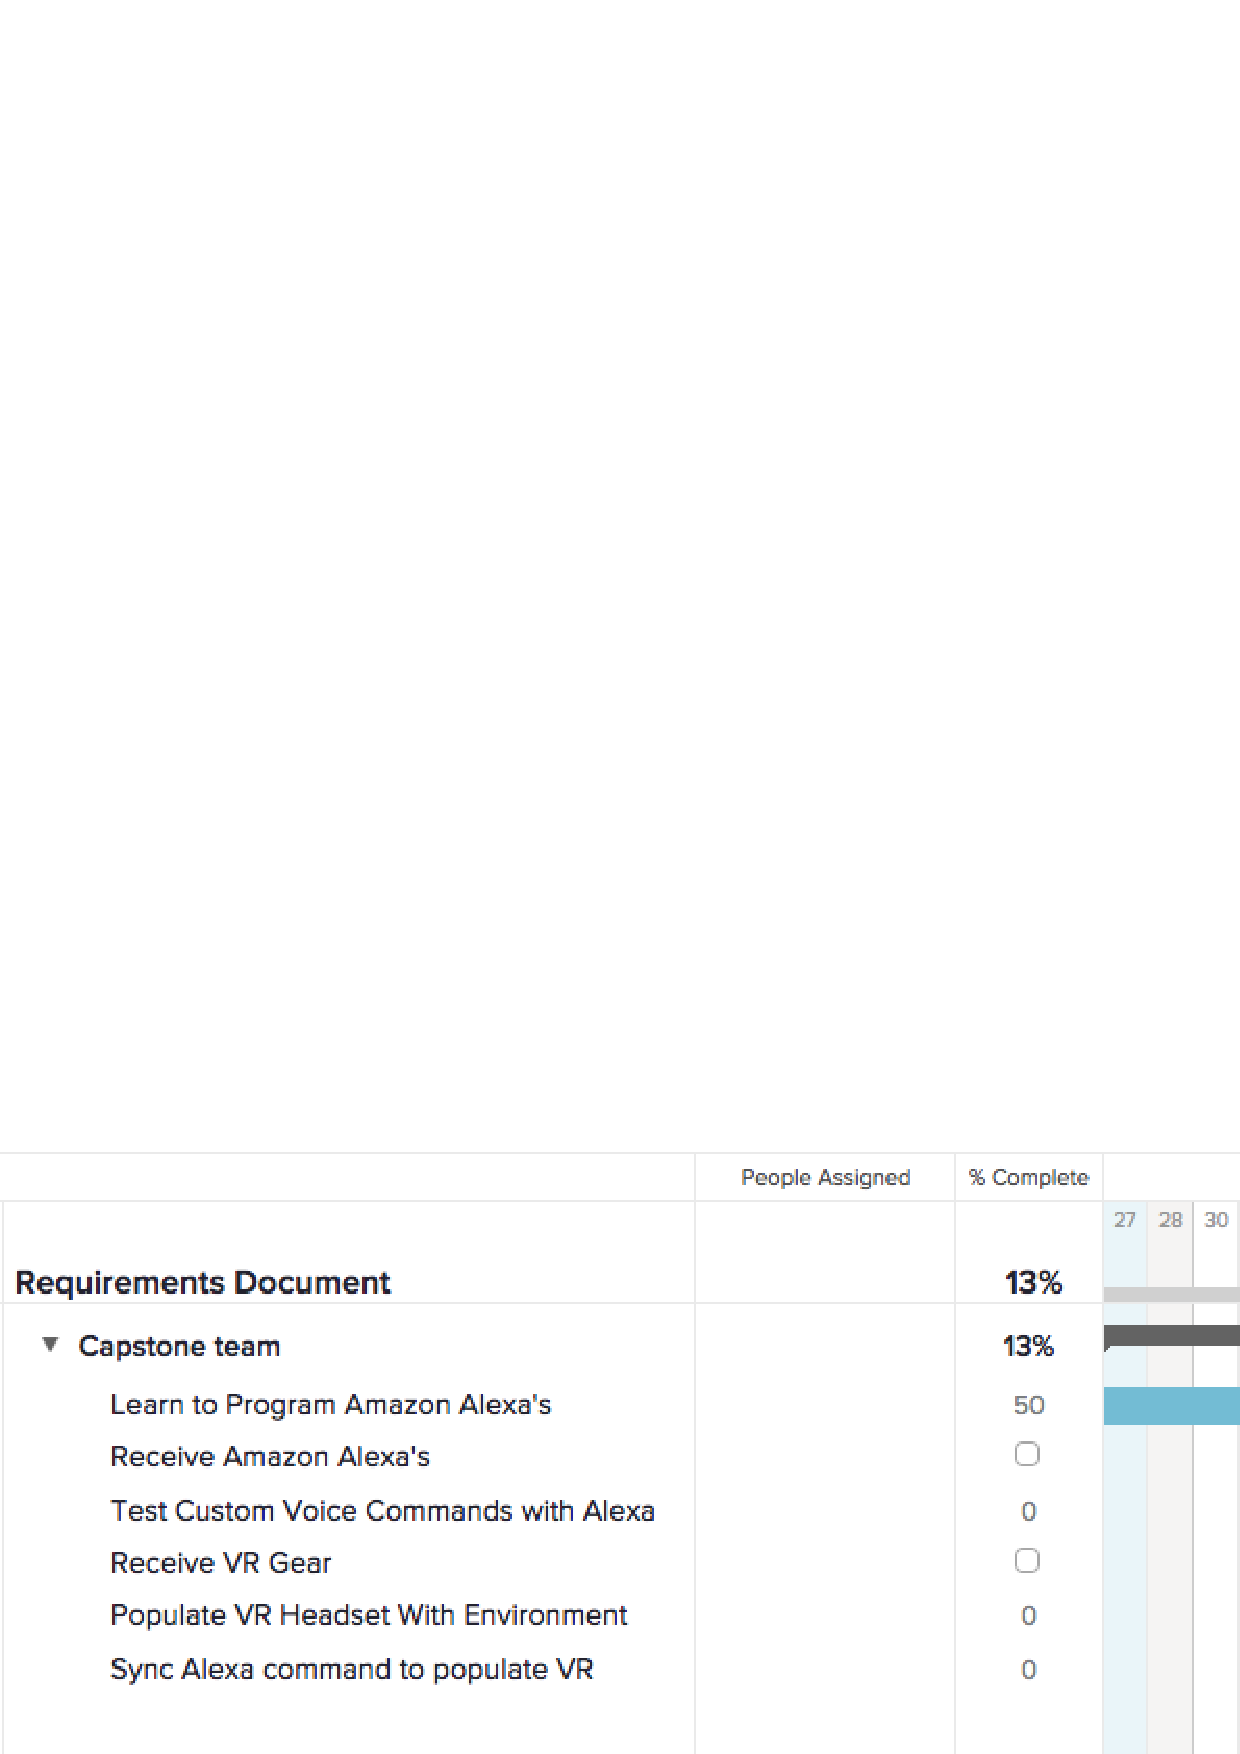
\includegraphics[width=\textwidth,height=5cm]{Gantt.png}


\end{document}